\chapter{Reducing special ILPs to Shortest Path}
\section{Problem statement}
In their book \textit{Algebraic statistics for computational biology} \cite{algebraic_statistics}, the authors briefly mention an algorithm to solve integer linear programs by constructing a certain graph and solving the shortest path problem between two specifically chosen vertices. The resulting path will dictate the solution vector, and the length of that path will represent the value of that solution. Initially, this approach was restricted to matrices whose columns all sum up to the same number. In this chapter, we aim to revisit and rigorously explain this result. Furthermore, to enhance the practical feasibility of this algorithm, we will present some ideas to accelerate its execution.

\section{Solving Shortest Path using Dijkstra's Algorithm}
Before delving into the translation of Integer Linear Programs (ILPs) to a shortest path problem, let's revisit the fundamental concept of finding the shortest path in a graph. Dijkstra's algorithm stands as a cornerstone in graph theory, offering a systematic approach to determine the shortest path between nodes in a weighted graph \cite{introduction_to_algorithms}. It works by iteratively selecting the vertex with the shortest distance from the source and relaxing its outgoing edges. Here's how it works:

Given a weighted graph $G = (V, E)$ with vertices $V$ and edges $E$, and two specified vertices $s$ (source) and $t$ (target), we aim to find the shortest path from $s$ to $t$. Let $w(u, v)$ denote the weight of the edge from vertex $u$ to vertex $v$.

\begin{enumerate}
    \item Initialize a priority queue $Q$ and an array $dist$ to keep track of the shortest distance from the source vertex $s$ to every other vertex in the graph. Initially, set $dist[v] = \infty$ for all vertices $v$, except for $dist[s] = 0$.
    \item Enqueue the source vertex $s$ into the priority queue $Q$ with priority $0$.
    \item While $Q$ is not empty:
    \begin{enumerate}
        \item Dequeue a vertex $u$ with the minimum priority from $Q$.
        \item For each neighbor $v$ of $u$:
        \begin{enumerate}
            \item Calculate the potential new shortest distance to $v$ as $new\_dist = dist[u] + w(u, v)$.
            \item If $new\_dist < dist[v]$, update $dist[v]$ to $new\_dist$ and enqueue $v$ into $Q$ with priority $new\_dist$.
        \end{enumerate}
    \end{enumerate}
    \item Once the target vertex $t$ is dequeued from $Q$, the shortest path has been found, and the shortest distance to $t$ is $dist[t]$.
\end{enumerate}

The runtime complexity of Dijkstra's algorithm is $O((|V| + |E|) \log |V|)$ using a binary heap priority queue implementation. This makes it efficient for finding the shortest path in large, weighted graphs.


\section{Reduction}
\subsection{Definitions and preparation}
As previously stated, we will only be dealing with matrices in which all columns add up to the same value. To simplify, let's define an abbreviation:

\begin{definition}
    \label{def:CCS}
    Let $\mathbb{K}$ be a field and $\alpha \in \mathbb{K}$. Let $S_{\alpha}(\mathbb{K}^{m \times n})$ be the set of matricies of size $m \times n$, who's column all sum up to $\alpha$, namely:
    $$S_{\alpha}(\mathbb{K}^{m \times n}) := \{A \in \mathbb{K}^{m \times n}\mid \forall j \in [n]\colon \sum_{i=1}^{m} A_{ij} = \alpha\}$$
    We will call these matricies \textbf{CCS matricies}, for \textbf{C}onstant \textbf{C}olumn \textbf{S}um.
\end{definition}

ILPs are based on a system of linear equations, specifically $A \vec{x} = \vec{b}$. It is important to note that if $A$ is a CCS matrix, all solutions for $\vec{x}$ have specific properties, as described in the first lemma. This understanding is crucial for constructing the graph, which is our goal.

\begin{lemma}
    \label{lemma:ilp_pre1}
    Let $A\in S_\alpha(\N^{m \times n})$, $\alpha > 0$. Let $\vec b \in \N^m$ arbitrary and consider the linear system of equation $A\vec x=\vec b$, where $\vec x \in \N^n$. Then, the following two statements are true

    \begin{enumerate}
        \item[(1)] For all solutions $\vec x \in \N^n$ must hold that its components must always sum up to the same number $k$.
        \item[(2)] There only exist a solution of the components of $b$ sum up to a multiple of $\alpha$. This multiple turnes out to be $k \cdot \alpha$.
    \end{enumerate}
\end{lemma}

\begin{proof}
    Let's assume there exists a solution $\vec x \in \N^n$ of the linear system of equation $A\vec x=\vec b$.
    $$\sum_{i=1}^m b_i = \sum_{i=1}^{m}\sum_{j=1}^{n}A_{ij} x_j = \sum_{j=1}^{n}\underbrace{\sum_{i=1}^{m}A_{ij}}_\alpha x_j = \alpha \cdot \sum_{j=1}^{n}x_j$$
    Because $\alpha$ and $b_i$ are fixed and will not change dependent of $\vec x$ and $\alpha \neq 0$, statement (1) immidiatly follows. Thus we have proven, if there exist a solution $\vec x \in \N^n$, then it must hold that $\sum_{i=1}^{m}b_i = \alpha \cdot k$, which is the contraposition of (2).
\end{proof}


\subsection{Construction the graph}
\label{chap:graph_constrition}
We want to be able to solve an ILP by using the shortest path framework. The main task is to build a weighted, directed graph $G = (V, E)$ based on an ILP. As mentioned before, we will only look at ILPs who's matrix is a CCS matrix, let's call those CCS ILPs. Let $(A \in S_\alpha(\N^{m \times n}), \vec b \in \N^m, \vec\omega \in \Z^n), \alpha > 0$ be our ILP. Let $k := \frac{1}{\alpha} \sum_{i=1}^{n}b_i \in \N$. Because of lemma \ref{lemma:ilp_pre1}, $k \in \N$. Now we can build the set of vertecies $V$. The resulting graph consists of $k$ layers of vertecies. We will call the layers $V_i, i \in [k]$. Thus $V := V_1 \cup \dots \cup V_k$. Each vertex will be represented by some vector:
$$V_i := \left\{A\vec x \mid \vec x \in \N^n, \sum_{j=1}^{n} x_j = i \right\}$$ 
It is clear that $V_0 = \{\vec 0\}$ and if $A\vec x = \vec b$ has solutions, we know from lemma \ref{lemma:ilp_pre1} that $\vec b \in V_k$. 

Edges, will only exist between consecutive layers. The basic idea is, that the underlying connected vectors $\vec x, \vec x'$ will differ by some unit vector $\hat e$ ($\vec x' = \vec x + \hat e$). Only if this is true, the vertecies $A\vec x$ and $A\vec x'$ are connected. This can of cause only happen for vertecies in consecutive layers. More formally: 
$$E := \{(u, v) \in V^2\mid \exists \hat e \in \{\hat e_1, \dots, \hat e_n\}\colon v = u + A\hat e\}$$

The last steps is defining the weights of the graph. Remember that every edge corresponds to adding some unit vector. The dot-product of this unit vector and the weights vector will be the weight of that edge:
$$w(v, v + A\hat e_i) := \sprod{\vec \omega}{\hat e_i}$$

Now consider a path beween $\vec 0\in V_0$ and $\vec b \in V_k$. As edges only exist between consecutive layers, the path will always traverse exactly $k$ edges and therby visit all $k+1$ layers once.

The next lemma will link paths in $G$ to our ILP, which will be essential when understanding why the shortest path solves our ILP.

\begin{lemma}
    Let $V, E, w, (A, \vec b, \vec \omega)$ be as in this chapter. Let $v \in V$ be a vertex of $G$. For any vector $\vec x \in \N^n$ such that $A\vec x = v$ there will be a path $P$ from $\vec 0$ to $v$ in $G$ such that the weight of $P$ is equal to $\sprod{\vec\omega}{\vec x}$. 
\end{lemma}
\begin{proof}
    We will prove, that this fact is true for any node in layer $i$, by induction over $i$. 
    
    The base case is $i=0$, hence we only have to consider $V_0$. We already know that $V_0 = \{\vec0\}$. So let $v := \vec 0$. The only vector $\vec x$ such that $A\vec x = v$ is $\vec x = \vec 0$, the column sums in $A$ are strictly positive. Thus $\sprod{\vec x}{\omega} = 0$ and the only path from $\vec 0$ to $\vec 0$ is the empty path with weight 0. Tadaa
    
    Let the statement be true for some $i < k$. We will proof it for $i+1$. Let $v \in V_{i+1}$ and $\vec x \in \N^n$ such that $A\vec x = v$. We know that $\sum_{j=1}^n x_j = i+1$. Let $\hat e$ be a basis vector such that $\vec x - \hat e =: \vec x' \in \N^n$. We know that $\sum_{j=1}^{n} x'_i = i+1-1=i$ and hence $A\vec x' \in V_i$. Thus by assumption there exists a path $P'$ from $\vec 0$ to $v' := A\vec x'$ such that its weight is $\sprod{\vec \omega}{\vec x'}$. Because $\vec x$ and $\vec x'$ only differ by a unit vector $\hat e$, the edge $(v', v)$ exists with weight $A\hat e$. So we can consider the path $P := P' \circ (v', v)$. It connects $\vec 0$ and $v$. And has the weight of $P'$ plus the weight of the edge, thus the weight $\sprod{\vec \omega}{\vec x'} + \sprod{\vec\omega}{\hat e} = \sprod{\vec \omega}{\vec x' + \hat e} = \sprod{\vec \omega}{\vec x}$. Which proves what we wanted to show.
\end{proof}

Hence, looking at all paths from $\vec 0$ to $\vec b$ and then considering their weights is equivilant to looking at all solution to $A\vec x = \vec b$ and considering all values $\sprod{\vec\omega}{\vec x}$. The shortest path represents the smallest of those values. Hence solving shortest path between $\vec 0$ and $\vec b$ will yield a path who's weight is the optimal value for $\sprod{\vec\omega}{\vec x}$.\qed

An example of this graph construction can be viewed in figure \ref{fig:ILP2graph_no_optimisation}
\begin{figure}
    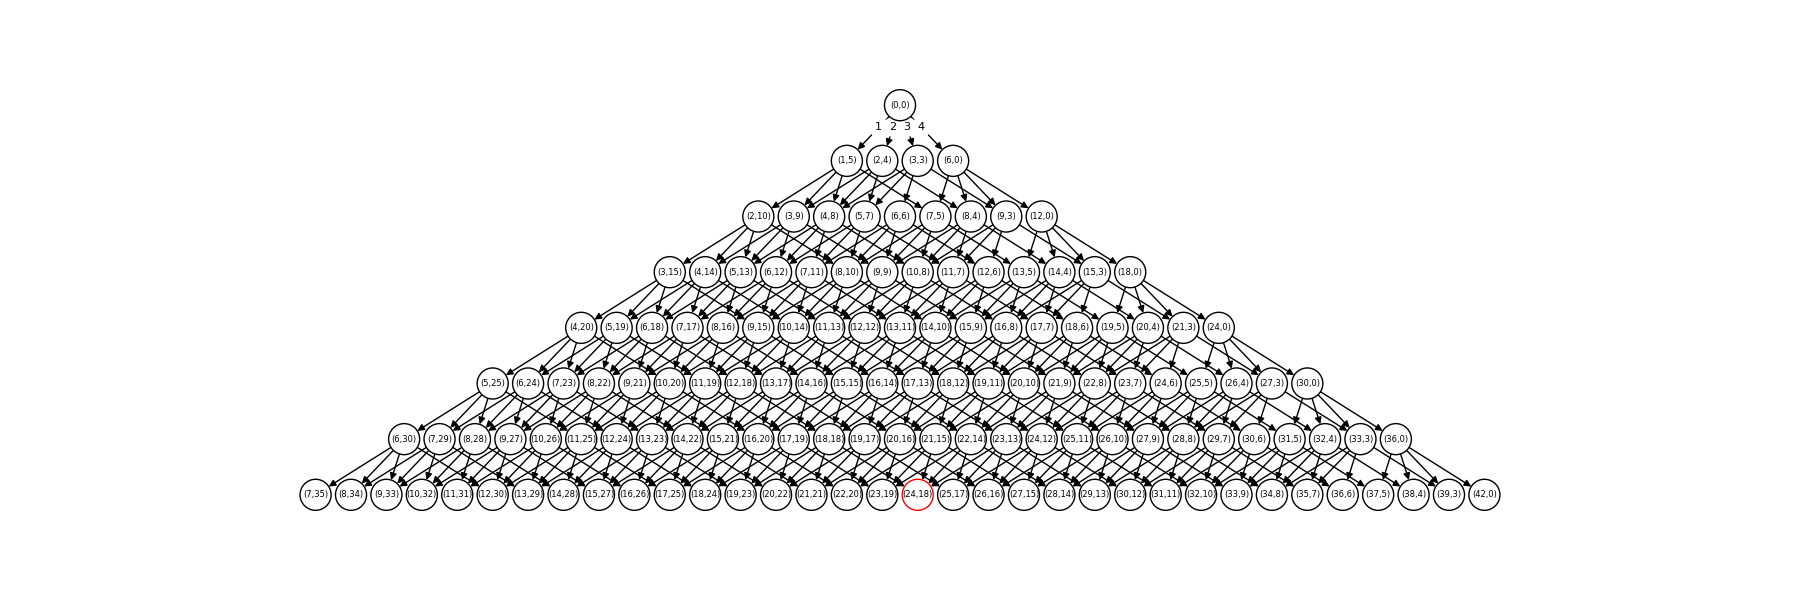
\includegraphics[width=\columnwidth]{ILP2graph.png}
    \caption{\label{fig:ILP2graph_no_optimisation}The graph for the ILP: $A = \smat{1&2&3&6\\5&4&3&0}, \vec b = \smat{24\\18}, \vec \omega = \smat{1\\2\\3\\4}$. All weights after the first layer are hidden.}
\end{figure}

\section{Immediate optimisation ideas}
\label{chap:graph_optimisation}
As shown, the graphs can quickly become large due to the NP-hard nature of ILPs. However, there are ways to reduce the size of the graph. Firstly, note that the entries in the vertex vectors can only increase when moving down the layers. Therefore, if at least one entry is larger than the corresponding entry in vector b, we can remove the node or stop considering it in Dijkstra's algorithm. After removing the larger nodes, the graph becomes significantly smaller, as shown in figure \ref{fig:ILP2graph_no_big_entries}.

\begin{figure}
    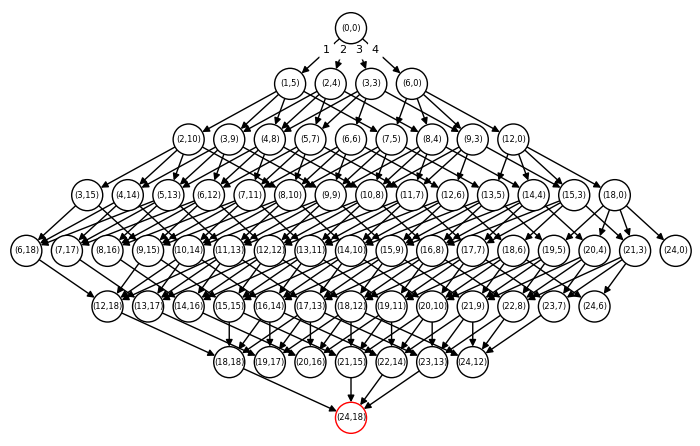
\includegraphics[width=\columnwidth]{ILP2graph_no_big_entries.png}
    \caption{\label{fig:ILP2graph_no_big_entries}The graph for the ILP: $A = \smat{1&2&3&6\\5&4&3&0}, \vec b = \smat{24\\18}, \vec \omega = \smat{1\\2\\3\\4}$. All weights after the first layer are hidden. All vertecies have been removed, where at least one component is bigger than the corresponding one in $\vec b$}
\end{figure}

As well as removing vertices, we can also remove some edges. To see this, consider the node $A(\hat e_1 + \hat e_2)$. We know that it exists in layer 2. We can see that there are at least 2 paths from $\vec 0$ to this node, $\vec 0 \rightarrow A\hat e_1 \rightarrow A(\hat e_1 + \hat e_2)$ and $\vec 0 \rightarrow A\hat e_2 \rightarrow A(\hat e_1 + \hat e_2)$. And both paths will have the same weight, namely $\sprod{\vec \omega}{\hat e_1 + \hat e_2}$, and will also represent the same vector $\hat e_1 + \hat e_2$. The fact that there are 2 paths for a vector is redundant and negatively affects the performance of the shortest path search. We can remove these duplicate paths by remembering which unit vector we added prevously, let it be $\hat e_i$, and only add unit vectors $\hat e_j$ with $j \geq i$ to construct edges. Then the edge $(A\hat e_2, A(\hat e_1 + \hat e_2))$ would not exist and the duplicate path would be removed. Doing this on the original graph, you get the figure \ref{fig:ILP2graph_unique_paths}.

\begin{figure}
    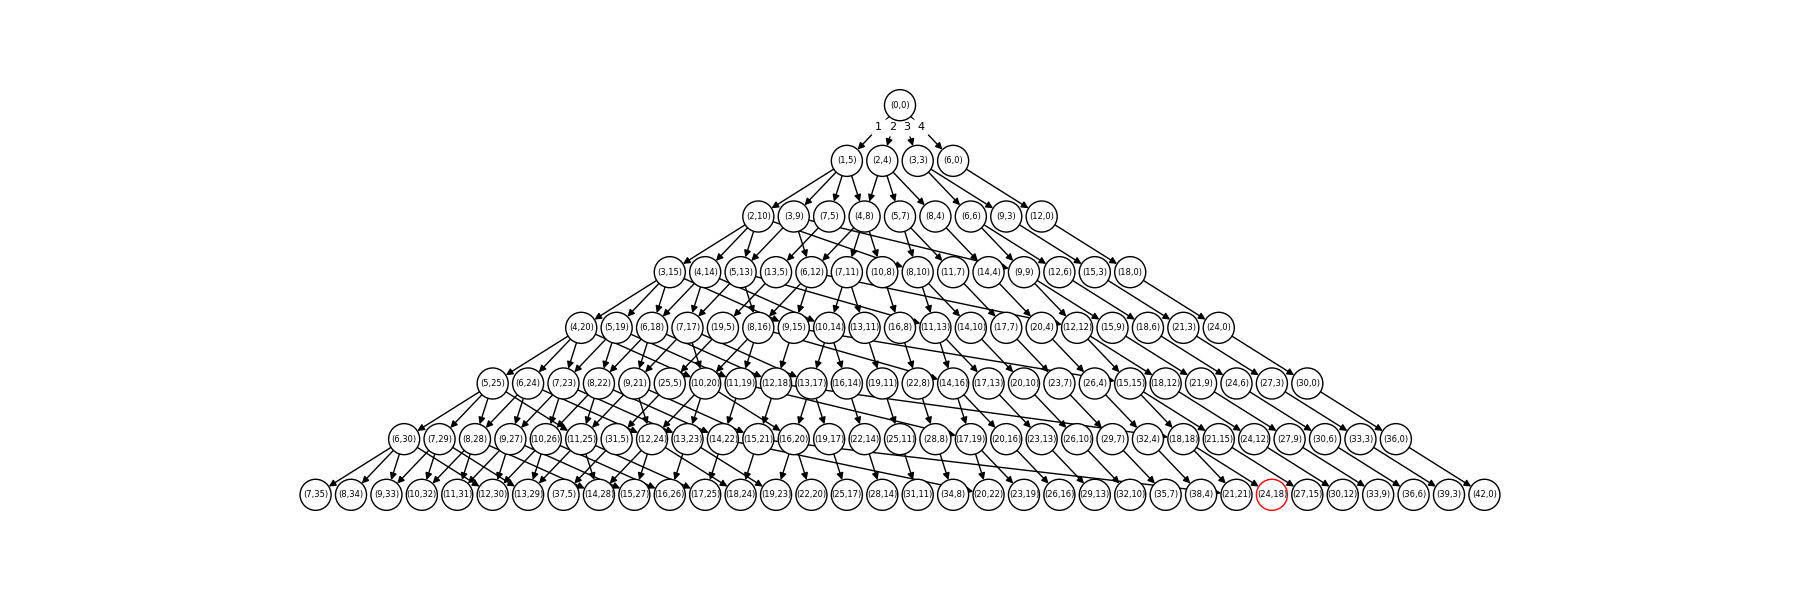
\includegraphics[width=\columnwidth]{ILP2graph_unique_paths.png}
    \caption{\label{fig:ILP2graph_unique_paths}The graph for the ILP: $A = \smat{1&2&3&6\\5&4&3&0}, \vec b = \smat{24\\18}, \vec \omega = \smat{1\\2\\3\\4}$. All vectors $\vec x$ now correspond with an \textit{unique} path from $\vec 0$ to $A\vec x$.}
\end{figure}

We have seen an option to remove vertices and an option to remove edges. But we do not need to apply these 2 optimisations separately, we can combine them. The result is a drastic reduction in the size of the graph, as shown in the figure \ref{fig:ILP2graph_unique_paths_and_no_big_entries}.

\begin{figure}
    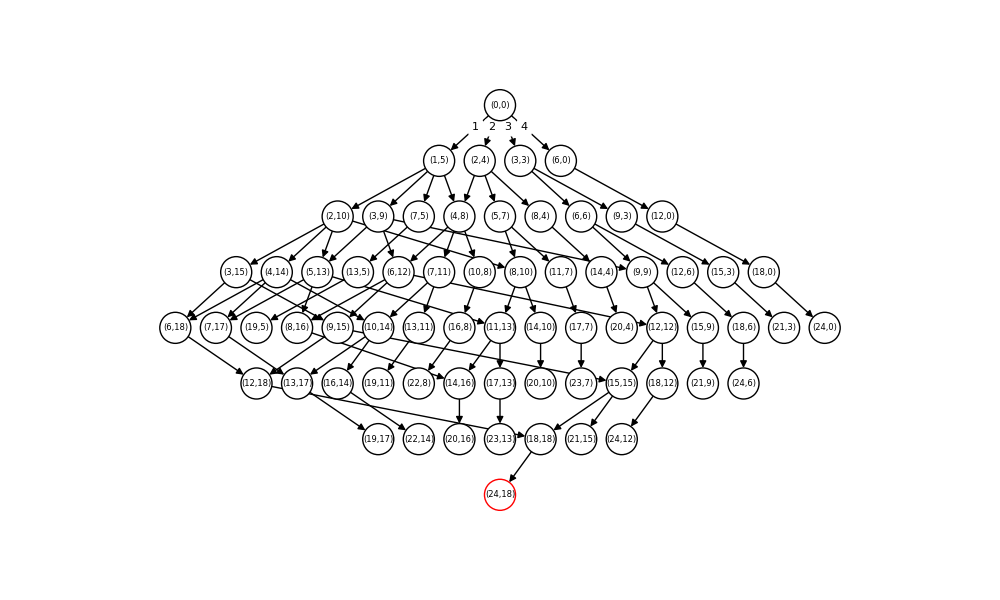
\includegraphics[width=\columnwidth]{ILP2graph_unique_paths_and_no_big_entries.png}
    \caption{\label{fig:ILP2graph_unique_paths_and_no_big_entries}The graph for the ILP: $A = \smat{1&2&3&6\\5&4&3&0}, \vec b = \smat{24\\18}, \vec \omega = \smat{1\\2\\3\\4}$. Unique paths and big components removed.}
\end{figure}

Looking at the final result in figure \ref{fig:ILP2graph_unique_paths_and_no_big_entries} you might say that it would be beneficial to remove the vertices without children. And yes, that would make the graph even smaller. The problem with this optimisation is that it can't be done on the fly within the Dajkstra algorithm. The vertecies can be discarded when they are visited, and the edges can be discarded when a vertex is processed. But whether a vertex has children or not cannot be known a priori. Nevertheless, I have included the graph when we iteratively - bottom up - remove all nodes without children to better understand the graph, see figure \ref{fig:ILP2graph_unique_paths_and_no_big_entries_and_no_leaves}.

\begin{figure}
    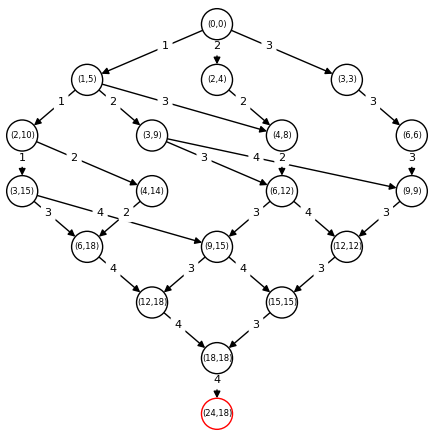
\includegraphics[width=\columnwidth]{ILP2graph_unique_paths_and_no_big_entries_and_no_leaves.png}
    \caption{\label{fig:ILP2graph_unique_paths_and_no_big_entries_and_no_leaves}The graph for the ILP: $A = \smat{1&2&3&6\\5&4&3&0}, \vec b = \smat{24\\18}, \vec \omega = \smat{1\\2\\3\\4}$. Unique paths and big components removed and all childrenless vertecies removed.}
\end{figure}

From this manageable representation we can read the solution of the ILP. The path with the lowest weight is the one on the far left of the graph. This path corresponds to $\vec x = \hat e_1 + \hat e_1 + \hat e_1 + \hat e_3 + \hat e_4 + \hat e_4 + \hat e_4 = (3, 0, 1, 3)^\top$ and indeed $A\vec x = \vec b$. 

